% This part is to be filled by Johann

% Feel free to change the amount of slides, this is just meant as a starting point

\begin{frame}{Goals}
  \begin{enumerate}
    \item Develop a CLI tool compatible with current state-of-the-art research
    \pause
    \item Performance and Efficiency
      \begin{itemize}
        \item Create a blazingly fast software package
        \item Provide a 100\% pure Rust alternative to classical solvers
        \item Support both shared and distributed memory parallelization
        \item Achieve full documentation coverage
        \item Achieve high unit test coverage
      \end{itemize}
  \end{enumerate}
\end{frame}
\begin{frame}{Goals (cont.)}
  \begin{enumerate}
      \setcounter{enumi}{2}
    \item Exact Solving
      \begin{itemize}
        \item Implement a simple, exact solver for the TSP
        \item Offer several optimized versions
        \item Create a shared memory parallelized verion
        \item Develop a distributed memory, MPI-based parallelized solver
      \end{itemize}
      \pause
    \item Approximation Tactics
      \begin{itemize}
        \item Include a trivial, easy to parallelize tactic and
        \item A sophisticated, state of the art tactic
        \item For both:
          \begin{itemize}
            \item Provide a shared memory parallelized solver
            \item Provide a distributed memory, MPI based parallelized solver
          \end{itemize}
      \end{itemize}
      \pause
    \item Lower Bound Calculation for TSP
      \begin{itemize}
        \item Provide a sequential implementation
        \item Develop a parallelized implementation using MPI
      \end{itemize}
  \end{enumerate}
\end{frame}

\begin{frame}{Organizational Remark}
  Targeted Credits for this course:
  \begin{itemize}
    \item Lars: 9C
    \item Johann: 6C
  \end{itemize}
~\\
  See also \url{https://hps.vi4io.org/_media/teaching/summer_term_2023/pchpc/pchpcassignment.pdf}
  for expected work depending on the targeted credits.
\end{frame}

% Or any other kind of information
\begin{frame}{Travelling Salesman Problem Definition}
\begin{minipage}{0.45\textwidth}
  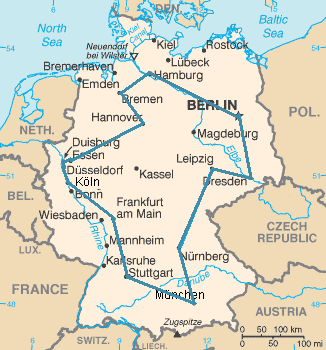
\includegraphics[width=0.8\textwidth]{TSP_Deutschland_3}
  \tiny

  user "Kapitän Nemo" \url{https://commons.wikimedia.org/w/index.php?curid=5584283}
\end{minipage}
\begin{minipage}{0.45\textwidth}

"Given a list of cities and the distances between each pair of cities, what is the shortest possible route that visits each city exactly once and returns to the origin city?"
\cite{song_solving_2021}
\end{minipage}
\end{frame}

\begin{frame}{Travelling Salesman Problem Definition}
  \begin{itemize}
    \item input graph
      \begin{itemize}
        \item weighted, non-negative
        \item undirected
        \item complete (fully connected)
      \end{itemize}

    \pause
    \item output restrictions:
      \begin{itemize}
        \item tour (cycle that visits every vertex)
        \item use any edge \emph{at most} one time
      \end{itemize}
    \pause
    \item problem: find a legal output that has minimal (cumulative) edge weight
  \end{itemize}
\end{frame}

\begin{frame}{Why is TSP interesting?}
  \begin{itemize}
    \item well studied
    \item NP-complete $\rightarrow$ ressource intensive
    \item intuitive to understand
    \pause
    \item practical applications (see \href{https://en.wikipedia.org/wiki/Concorde_TSP_Solver}{Concorde TSP Solver})
  \end{itemize}
  % https://upload.wikimedia.org/wikipedia/commons/c/c4/TSP_Deutschland_3.png
\end{frame}

\begin{frame}{Our Implementation}
  \begin{itemize}
    \item Publicly available on GitHub
    \item can be found on at \url{https://crates.io/crates/walky/}
    \item licensed under the MIT open source license
  \end{itemize}
\end{frame}

%\begin{frame}{MST}
%\end{frame}
